% !TEX program = xelatex
\documentclass[12pt,a4paper]{report}

% ===================== PACKAGES =====================
\usepackage[a4paper,left=2.5cm,right=2.5cm,top=2.5cm,bottom=2.5cm]{geometry}
\usepackage{fontspec}
\setmainfont{Tinos}
\usepackage[french]{babel}
\usepackage{setspace}
\usepackage{graphicx}
\usepackage{float}
\usepackage{array}
\usepackage{longtable}
\usepackage{booktabs}
\usepackage{multirow}
\usepackage{caption}
\usepackage{hyperref}
\usepackage{xcolor}
\usepackage{titlesec}
\usepackage{fancyhdr}
\usepackage{enumitem}
\usepackage{listings}
\usepackage{amsmath}
\usepackage{tikz}
\usetikzlibrary{positioning,arrows.meta,shapes.geometric}

\graphicspath{{../figures/}{figures/}}
\onehalfspacing
\setlength{\parindent}{0.8cm}
\setlength{\parskip}{6pt}
\setlength{\headheight}{15pt}
\sloppy

% ===================== MISE EN FORME =====================
\titleformat{\chapter}{\normalfont\bfseries\fontsize{16}{18}\selectfont\color{black}}{\thechapter.}{1em}{}
\titleformat{\section}{\normalfont\bfseries\fontsize{14}{16}\selectfont\color{black}}{\thesection}{1em}{}
\titleformat{\subsection}{\normalfont\bfseries\fontsize{12}{14}\selectfont\color{black}}{\thesubsection}{1em}{}

\captionsetup{font=small,labelfont=bf}

\hypersetup{
    colorlinks=true,
    linkcolor=black,
    urlcolor=blue,
    citecolor=black
}

\pagestyle{fancy}
\fancyhf{}
\fancyhead[L]{Rapport de stage}
\fancyhead[R]{TEACHIUM AI Tutor}
\fancyfoot[C]{\thepage}

\lstdefinestyle{pythonstyle}{
    language=Python,
    basicstyle=\ttfamily\small,
    numbers=left,
    numberstyle=\tiny,
    frame=single,
    breaklines=true,
    showstringspaces=false,
    tabsize=4
}

% ===================== DOCUMENT =====================
\begin{document}

% ===================== PAGE DE GARDE =====================
\begin{titlepage}
    \centering
    \vspace*{1cm}
    {\Large \textbf{Ecole Marocaine des Sciences de l'Ingénieur de Tanger}}\\[0.6cm]
    {\large 1ère Année Cycle d'Ingénieur}\\[0.4cm]
    {\large Filière : Ingénierie Informatique et Réseaux}\\[1.2cm]
    
    {\Huge \textbf{Rapport de Stage}}\\[0.6cm]
    {\Large \textbf{Entreprise d'accueil : TEACHIUM}}\\[1.2cm]
    
    \rule{\linewidth}{0.5mm}\\[0.5cm]
    {\Large \textbf{Développement d'un système de tutorat intelligent basé sur l'IA pour la personnalisation des parcours d'apprentissage}}\\[0.5cm]
    \rule{\linewidth}{0.5mm}\\[1.5cm]
    
    \begin{flushleft}
    \large
    \textbf{Réalisé par :} Mohamed Ben Yahya\\[0.3cm]
    \textbf{Organisme d'accueil :} TEACHIUM\\[0.3cm]
    \textbf{Localisation :} Tétouan, Tanger-Tétouan-Al Hoceïma, Maroc\\[0.3cm]
    \textbf{Durée du stage :} 1 mois\\[0.3cm]
    \textbf{Tuteur pédagogique :} À compléter\\[0.3cm]
    \textbf{Tuteur dans l'entreprise :} À compléter\\[0.3cm]
    \textbf{Année universitaire :} 2025--2026
    \end{flushleft}
    
    \vfill
    {\large Juillet 2026}
\end{titlepage}

% ===================== REMERCIEMENTS =====================
\pagenumbering{Roman}
\chapter*{Remerciements}
\addcontentsline{toc}{chapter}{Remerciements}

Je tiens à exprimer mes sincères remerciements à l'entreprise TEACHIUM pour m'avoir accueilli dans le cadre de ce stage et pour m'avoir donné l'opportunité de travailler sur un sujet actuel combinant e-learning, intelligence artificielle et développement logiciel.

Je remercie également mon encadrant professionnel pour son accompagnement, ses orientations et ses remarques qui m'ont permis de mieux comprendre les besoins réels d'une plateforme d'apprentissage numérique. Mes remerciements s'adressent aussi à mon encadrant pédagogique pour son suivi et ses conseils méthodologiques tout au long de cette expérience.

Enfin, je remercie toutes les personnes qui ont contribué directement ou indirectement à la réalisation de ce travail.

% ===================== RESUME =====================
\chapter*{Résumé}
\addcontentsline{toc}{chapter}{Résumé}

Ce rapport présente le travail réalisé dans le cadre d'un stage d'un mois au sein de l'entreprise TEACHIUM, spécialisée dans le développement de contenus e-learning et de solutions d'apprentissage numérique. Le projet porte sur la conception et le développement d'un système de tutorat intelligent basé sur l'intelligence artificielle afin de personnaliser les parcours d'apprentissage des apprenants.

La solution proposée repose sur l'analyse des données d'apprentissage, la modélisation des profils apprenants à l'aide de techniques de machine learning, la génération de recommandations pédagogiques personnalisées, l'intégration d'un assistant conversationnel simple et l'exposition des fonctionnalités via une API REST. Un tableau de bord a également été développé afin de visualiser les indicateurs pédagogiques et les performances des modèles.

Le prototype réalisé utilise un dataset simulé, un algorithme K-Means pour le regroupement des apprenants, un arbre de décision pour la classification des profils, un moteur de recommandation basé sur des règles pédagogiques et une interface de suivi développée avec Streamlit. Les résultats obtenus montrent la faisabilité d'une première version fonctionnelle adaptée à la durée limitée du stage.

\textbf{Mots clés :} e-learning, intelligence artificielle, tutorat intelligent, machine learning, recommandation, API REST, dashboard.

% ===================== ABSTRACT =====================
\chapter*{Abstract}
\addcontentsline{toc}{chapter}{Abstract}

This report presents the work carried out during a one-month internship at TEACHIUM, a company specialized in e-learning content development and digital learning solutions. The project focuses on designing and developing an AI-based intelligent tutoring system for personalizing learning paths.

The proposed solution is based on learning data analysis, learner profile modeling using machine learning techniques, personalized pedagogical recommendation, a simple conversational assistant, and REST API integration. A dashboard was also developed to visualize learning indicators and model performance.

The prototype uses a simulated dataset, K-Means clustering for learner grouping, a decision tree model for profile classification, a rule-based recommendation engine, and a Streamlit dashboard. The obtained results demonstrate the feasibility of a first functional version adapted to the limited internship duration.

\textbf{Key words:} e-learning, artificial intelligence, intelligent tutoring system, machine learning, recommendation, REST API, dashboard.

\tableofcontents
\listoffigures
\listoftables

\chapter*{Liste des abréviations}
\addcontentsline{toc}{chapter}{Liste des abréviations}
\begin{longtable}{|p{3cm}|p{11cm}|}
\hline
\textbf{Abréviation} & \textbf{Signification} \\
\hline
API & Application Programming Interface \\
\hline
BI & Business Intelligence \\
\hline
IA & Intelligence Artificielle \\
\hline
LLM & Large Language Model \\
\hline
LMS & Learning Management System \\
\hline
ML & Machine Learning \\
\hline
MVP & Minimum Viable Product \\
\hline
NLP & Natural Language Processing \\
\hline
REST & Representational State Transfer \\
\hline
UML & Unified Modeling Language \\
\hline
\end{longtable}

% ===================== INTRODUCTION =====================
\cleardoublepage
\pagenumbering{arabic}
\chapter*{Introduction générale}
\addcontentsline{toc}{chapter}{Introduction générale}

L'évolution rapide des technologies numériques a profondément transformé le domaine de la formation. Les plateformes e-learning permettent aujourd'hui aux apprenants d'accéder à des contenus pédagogiques à distance, de suivre des modules de formation, de passer des quiz et de consulter leur progression. Toutefois, plusieurs plateformes proposent encore des parcours relativement uniformes, sans adaptation suffisante au niveau, au rythme et aux difficultés de chaque apprenant.

Dans ce contexte, l'intelligence artificielle représente une opportunité importante pour améliorer la personnalisation de l'apprentissage. En analysant les données générées par les apprenants, il devient possible d'identifier des profils pédagogiques, de détecter les besoins individuels, de recommander des contenus adaptés et d'accompagner l'utilisateur à travers une assistance conversationnelle.

Le présent stage, réalisé au sein de TEACHIUM, porte sur le développement d'un système de tutorat intelligent basé sur l'IA. Le projet vise à proposer un prototype fonctionnel capable d'analyser les profils apprenants, de générer des recommandations personnalisées, de fournir un assistant conversationnel simple et d'intégrer ces fonctionnalités dans une architecture applicative à travers une API REST.

La problématique principale peut être formulée comme suit : comment concevoir un système intelligent capable d'exploiter les données d'apprentissage pour personnaliser les parcours pédagogiques des utilisateurs d'une plateforme e-learning ?

Les objectifs du projet sont donc multiples. Il s'agit d'abord de préparer des données exploitables, ensuite de modéliser les profils apprenants à l'aide du machine learning, puis de concevoir un moteur de recommandation et un assistant intelligent. Enfin, il faut intégrer ces modules dans un système applicatif simple, testable et présentable.

Ce rapport est structuré en cinq chapitres. Le premier chapitre présente l'entreprise d'accueil et la mission de stage. Le deuxième chapitre détaille le cahier des charges et le déroulement du stage. Le troisième chapitre expose l'étude bibliographique et les notions nécessaires. Le quatrième chapitre présente la conception du système. Le cinquième chapitre décrit l'implémentation, les tests et les résultats obtenus.

% ===================== CHAPITRE 1 =====================
\chapter{Entreprise d'accueil et mission}

\section{Présentation de l'entreprise}

TEACHIUM est une entreprise spécialisée dans le domaine de l'apprentissage numérique et du développement de contenus e-learning. Elle accompagne les organisations dans la conception de solutions de formation digitales et dans l'utilisation de la technologie pour améliorer les performances d'apprentissage.

L'entreprise est localisée à Tétouan, dans la région Tanger-Tétouan-Al Hoceïma. Elle opère dans le secteur des programmes d'éducation et de formation, avec des spécialités liées au développement de contenus e-learning, aux solutions de formation, à l'expertise en apprentissage numérique et aux systèmes de gestion de l'apprentissage.

\begin{table}[H]
\centering
\caption{Fiche synthétique de TEACHIUM}
\begin{tabular}{|p{5cm}|p{9cm}|}
\hline
\textbf{Élément} & \textbf{Description} \\
\hline
Nom de l'entreprise & TEACHIUM \\
\hline
Secteur & Éducation, e-learning et solutions de formation numérique \\
\hline
Localisation & Tétouan, Tanger-Tétouan-Al Hoceïma, Maroc \\
\hline
Année de création & 2010 \\
\hline
Taille & Petite structure, environ 2 à 10 employés \\
\hline
Spécialités & E-learning content development, e-learning expertise, learning solutions, LMS \\
\hline
Site web & \url{https://www.teachium.com} \\
\hline
\end{tabular}
\end{table}

\section{Domaine d'activité}

Le domaine d'activité de TEACHIUM se situe à l'intersection de la formation, de la technologie et de l'ingénierie pédagogique. L'entreprise propose des solutions destinées à faciliter la création, la gestion et la diffusion de contenus d'apprentissage numériques.

Dans ce type d'environnement, les données issues des interactions des apprenants peuvent avoir une grande valeur. Les scores, le temps passé, le taux de complétion, la fréquence de connexion et les feedbacks permettent de mieux comprendre les comportements d'apprentissage et d'améliorer la pertinence des parcours proposés.

\section{Mission confiée}

La mission confiée dans le cadre de ce stage est le développement d'un système de tutorat intelligent basé sur l'intelligence artificielle. Cette mission s'inscrit dans les besoins actuels des plateformes e-learning : accompagner les apprenants de manière personnalisée et fournir aux équipes pédagogiques des indicateurs de suivi pertinents.

La mission est organisée autour de quatre axes principaux :

\begin{enumerate}
    \item analyse et modélisation des profils apprenants ;
    \item conception d'un moteur de recommandation et d'une assistance conversationnelle ;
    \item intégration via une API REST et création d'un tableau de bord ;
    \item évaluation et optimisation des modèles IA.
\end{enumerate}

\section{Rôle dans l'équipe}

Dans le cadre du stage, le rôle principal consiste à concevoir et développer un prototype fonctionnel. Les tâches réalisées couvrent l'analyse du besoin, la préparation des données, le développement des modèles IA, la création du backend API, la conception du moteur de recommandation, le développement du dashboard et la préparation des livrables techniques.

% ===================== CHAPITRE 2 =====================
\chapter{Cahier des charges et déroulement du stage}

\section{Problématique}

Les apprenants n'ont pas tous le même niveau, le même rythme, ni les mêmes difficultés. Une plateforme qui propose le même parcours à tous les utilisateurs ne permet pas toujours d'accompagner efficacement chaque apprenant. Un apprenant en difficulté a besoin de révision et d'exercices guidés, tandis qu'un apprenant avancé a plutôt besoin de contenus plus complexes ou de projets pratiques.

La problématique du projet est donc la suivante : comment concevoir un système intelligent capable d'analyser les données d'un apprenant, d'identifier son profil pédagogique et de lui proposer un accompagnement adapté ?

\section{Objectifs du projet}

L'objectif général du projet est de développer un prototype de système de tutorat intelligent pour personnaliser les parcours d'apprentissage sur une plateforme e-learning.

Les objectifs spécifiques sont les suivants :

\begin{itemize}
    \item collecter ou simuler des données d'apprentissage exploitables ;
    \item analyser les comportements des apprenants ;
    \item regrouper les apprenants par profils à l'aide du clustering ;
    \item classifier les apprenants selon leur profil pédagogique ;
    \item générer des recommandations personnalisées ;
    \item proposer une assistance conversationnelle simple ;
    \item exposer les fonctionnalités via une API REST ;
    \item visualiser les indicateurs dans un tableau de bord ;
    \item évaluer les performances du prototype.
\end{itemize}

\section{Besoins fonctionnels}

\begin{longtable}{|p{2.5cm}|p{11.5cm}|}
\caption{Besoins fonctionnels du système}\\
\hline
\textbf{Code} & \textbf{Besoin fonctionnel} \\
\hline
\endfirsthead
\hline
\textbf{Code} & \textbf{Besoin fonctionnel} \\
\hline
\endhead
BF01 & Le système doit recevoir les données d'un apprenant. \\
\hline
BF02 & Le système doit analyser les indicateurs pédagogiques de l'apprenant. \\
\hline
BF03 & Le système doit identifier un profil pédagogique. \\
\hline
BF04 & Le système doit générer des recommandations adaptées au profil. \\
\hline
BF05 & Le système doit fournir une réponse conversationnelle simple. \\
\hline
BF06 & Le système doit exposer ses fonctionnalités via une API REST. \\
\hline
BF07 & Le système doit afficher les statistiques pédagogiques dans un dashboard. \\
\hline
BF08 & Le système doit fournir des métriques d'évaluation du modèle. \\
\hline
\end{longtable}

\section{Besoins non fonctionnels}

\begin{longtable}{|p{2.5cm}|p{11.5cm}|}
\caption{Besoins non fonctionnels du système}\\
\hline
\textbf{Code} & \textbf{Besoin non fonctionnel} \\
\hline
\endfirsthead
\hline
\textbf{Code} & \textbf{Besoin non fonctionnel} \\
\hline
\endhead
BNF01 & Le système doit être simple à utiliser et facile à tester. \\
\hline
BNF02 & L'architecture doit être claire et maintenable. \\
\hline
BNF03 & Les traitements doivent être suffisamment rapides pour un usage interactif. \\
\hline
BNF04 & Le code doit être organisé et documenté. \\
\hline
BNF05 & Les résultats doivent être interprétables pour un contexte pédagogique. \\
\hline
BNF06 & Le prototype doit pouvoir évoluer vers une intégration avec des données réelles. \\
\hline
\end{longtable}

\section{Déroulement du stage}

La durée du stage étant limitée à un mois, le travail a été organisé en quatre phases principales. La première semaine est consacrée à l'analyse du besoin et à la préparation des données. La deuxième semaine porte sur les modèles IA et le moteur de recommandation. La troisième semaine concerne l'intégration API REST et le dashboard. La dernière semaine est réservée aux tests, à l'optimisation et à la rédaction.

\begin{longtable}{|p{2.5cm}|p{5cm}|p{6cm}|}
\caption{Planning synthétique du stage}\\
\hline
\textbf{Période} & \textbf{Objectif} & \textbf{Livrables} \\
\hline
\endfirsthead
\hline
\textbf{Période} & \textbf{Objectif} & \textbf{Livrables} \\
\hline
\endhead
Semaine 1 & Cadrage et données & Cahier des charges, dataset, premières visualisations \\
\hline
Semaine 2 & IA et recommandation & Clustering, arbre de décision, moteur de recommandation, chatbot \\
\hline
Semaine 3 & Intégration & API REST, endpoints, dashboard \\
\hline
Semaine 4 & Validation & Tests, métriques, rapport, présentation \\
\hline
\end{longtable}

\section{Diagramme de Gantt}

\begin{longtable}{|p{4.5cm}|c|c|c|c|}
\caption{Diagramme de Gantt simplifié}\\
\hline
\textbf{Tâche} & \textbf{S1} & \textbf{S2} & \textbf{S3} & \textbf{S4} \\
\hline
\endfirsthead
\hline
\textbf{Tâche} & \textbf{S1} & \textbf{S2} & \textbf{S3} & \textbf{S4} \\
\hline
\endhead
Analyse du besoin & X & & & \\
\hline
Cahier des charges & X & & & \\
\hline
Préparation du dataset & X & & & \\
\hline
Analyse exploratoire & X & X & & \\
\hline
Clustering et classification & & X & & \\
\hline
Moteur de recommandation & & X & & \\
\hline
Assistant conversationnel & & X & X & \\
\hline
API REST & & & X & \\
\hline
Dashboard & & & X & \\
\hline
Tests et évaluation & & & & X \\
\hline
Rapport et présentation & & & & X \\
\hline
\end{longtable}

\section{Méthodologie de gestion}

La méthodologie adoptée est incrémentale. Chaque composant est développé sous forme de module indépendant, puis intégré progressivement dans le système complet. Cette approche est adaptée à un stage court, car elle permet d'obtenir rapidement un prototype démontrable tout en limitant les risques techniques.

% ===================== CHAPITRE 3 =====================
\chapter{Étude bibliographique}

\section{Systèmes de tutorat intelligent}

Un système de tutorat intelligent est un système informatique destiné à accompagner l'apprenant de manière personnalisée. Contrairement à un système d'apprentissage classique, il cherche à adapter les ressources, les exercices et les explications au profil de l'utilisateur. Dans le cadre de ce projet, l'adaptation repose sur les données d'apprentissage : scores, complétion, activité et feedback.

\section{Machine learning pour le profilage}

Le machine learning permet d'extraire des régularités à partir des données. Dans ce projet, deux familles de méthodes sont utilisées : les méthodes non supervisées et les méthodes supervisées.

Le clustering K-Means est utilisé pour regrouper automatiquement les apprenants selon leurs caractéristiques. La documentation officielle de scikit-learn présente K-Means comme un algorithme de regroupement paramétré notamment par le nombre de clusters et l'initialisation des centroïdes \cite{sklearn-kmeans}. Cette méthode est pertinente pour une première analyse de profils, car elle ne nécessite pas forcément des étiquettes prédéfinies.

L'arbre de décision est utilisé pour classifier les apprenants selon leur profil pédagogique. Dans scikit-learn, \texttt{DecisionTreeClassifier} permet de traiter des problèmes de classification binaire ou multiclasse \cite{sklearn-tree}. Ce modèle a été retenu parce qu'il est interprétable et adapté à une explication pédagogique des décisions.

\section{Moteur de recommandation pédagogique}

Un moteur de recommandation vise à proposer une ressource adaptée à un utilisateur. Dans ce projet, le moteur est volontairement simple et fondé sur des règles pédagogiques. Ce choix est justifié par la durée limitée du stage, le besoin d'interprétabilité et l'absence éventuelle de données réelles en grande quantité.

Par exemple, un apprenant en difficulté reçoit des cours de révision et des quiz de renforcement, tandis qu'un apprenant avancé reçoit des contenus plus complexes et des mini-projets. Ce moteur peut évoluer vers des techniques plus avancées si des historiques réels d'apprentissage deviennent disponibles.

\section{NLP, LLM et assistance conversationnelle}

Le traitement du langage naturel permet à un système de comprendre ou de générer du texte. Dans ce prototype, l'assistance conversationnelle reste simple : elle repose sur une détection de mots-clés et sur des réponses adaptées au profil de l'apprenant. Cette approche permet de démontrer l'utilité d'un assistant pédagogique sans dépendre d'un modèle coûteux.

Dans une version future, l'assistant pourrait être enrichi par une approche de type retrieval-augmented generation. Les travaux de Lewis et al. introduisent des modèles combinant une mémoire paramétrique et une mémoire non paramétrique récupérée par recherche documentaire, afin d'améliorer les tâches de NLP nécessitant des connaissances \cite{rag-lewis}. Une telle approche permettrait de répondre à partir des supports pédagogiques de TEACHIUM.

\section{API REST et dashboard}

FastAPI a été choisi pour exposer les fonctionnalités du système à travers une API REST. Le framework repose sur les standards ouverts OpenAPI et JSON Schema et fournit une documentation automatique des modèles de données \cite{fastapi-docs}. Cela facilite les tests via Swagger et l'intégration avec une plateforme e-learning.

Streamlit a été choisi pour créer rapidement un dashboard interactif en Python. La documentation officielle indique que Streamlit permet de construire des applications de données avec des graphiques, widgets et mises en page interactives \cite{streamlit-docs}. Ce choix est adapté au prototype, car il réduit le temps nécessaire au développement frontend.

% ===================== CHAPITRE 4 =====================
\chapter{Vue conceptuelle}

\section{Architecture générale du système}

Le système proposé est organisé autour de quatre couches : données, intelligence artificielle, API REST et interface de visualisation. La couche données contient les informations liées aux apprenants. La couche IA analyse les profils et génère les recommandations. La couche API rend les fonctionnalités accessibles. La couche interface permet de visualiser les statistiques et de tester le prototype.

\begin{figure}[H]
\centering
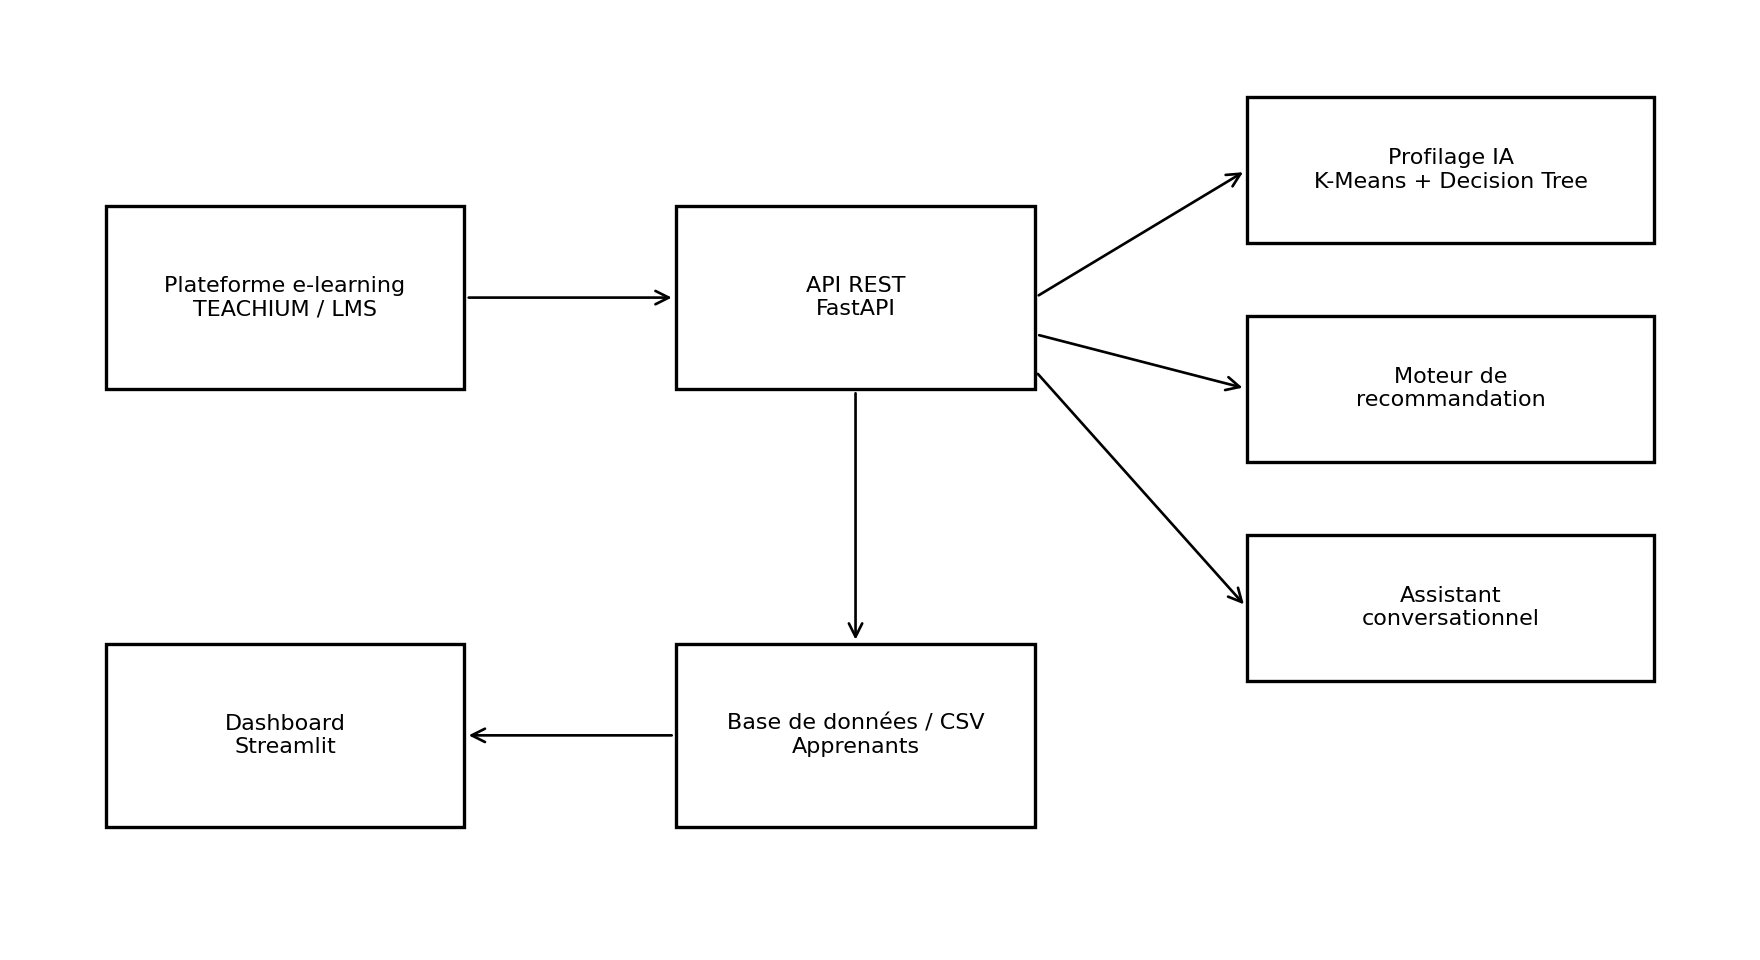
\includegraphics[width=0.95\textwidth]{architecture_systeme.png}
\caption{Architecture générale du système de tutorat intelligent}
\end{figure}

La figure précédente montre le flux principal du système. La plateforme e-learning ou un utilisateur envoie les données à l'API REST. L'API appelle les services IA, notamment le modèle de profilage, le moteur de recommandation et l'assistant conversationnel. Les données et les résultats sont ensuite visualisés dans le dashboard.

\section{Composants du système}

\begin{longtable}{|p{4cm}|p{10cm}|}
\caption{Composants principaux du système}\\
\hline
\textbf{Composant} & \textbf{Rôle} \\
\hline
\endfirsthead
\hline
\textbf{Composant} & \textbf{Rôle} \\
\hline
\endhead
Dataset apprenant & Contient les indicateurs pédagogiques utilisés par les modèles IA. \\
\hline
Profile Service & Analyse les données et retourne un profil pédagogique. \\
\hline
Recommendation Service & Génère une liste de ressources adaptées au profil. \\
\hline
Chatbot Service & Répond à des questions simples liées au profil ou aux recommandations. \\
\hline
FastAPI Controller & Expose les endpoints REST du système. \\
\hline
Dashboard Service & Affiche les statistiques et permet de tester le prototype. \\
\hline
\end{longtable}

\section{Diagramme de cas d'utilisation}

\begin{figure}[H]
\centering
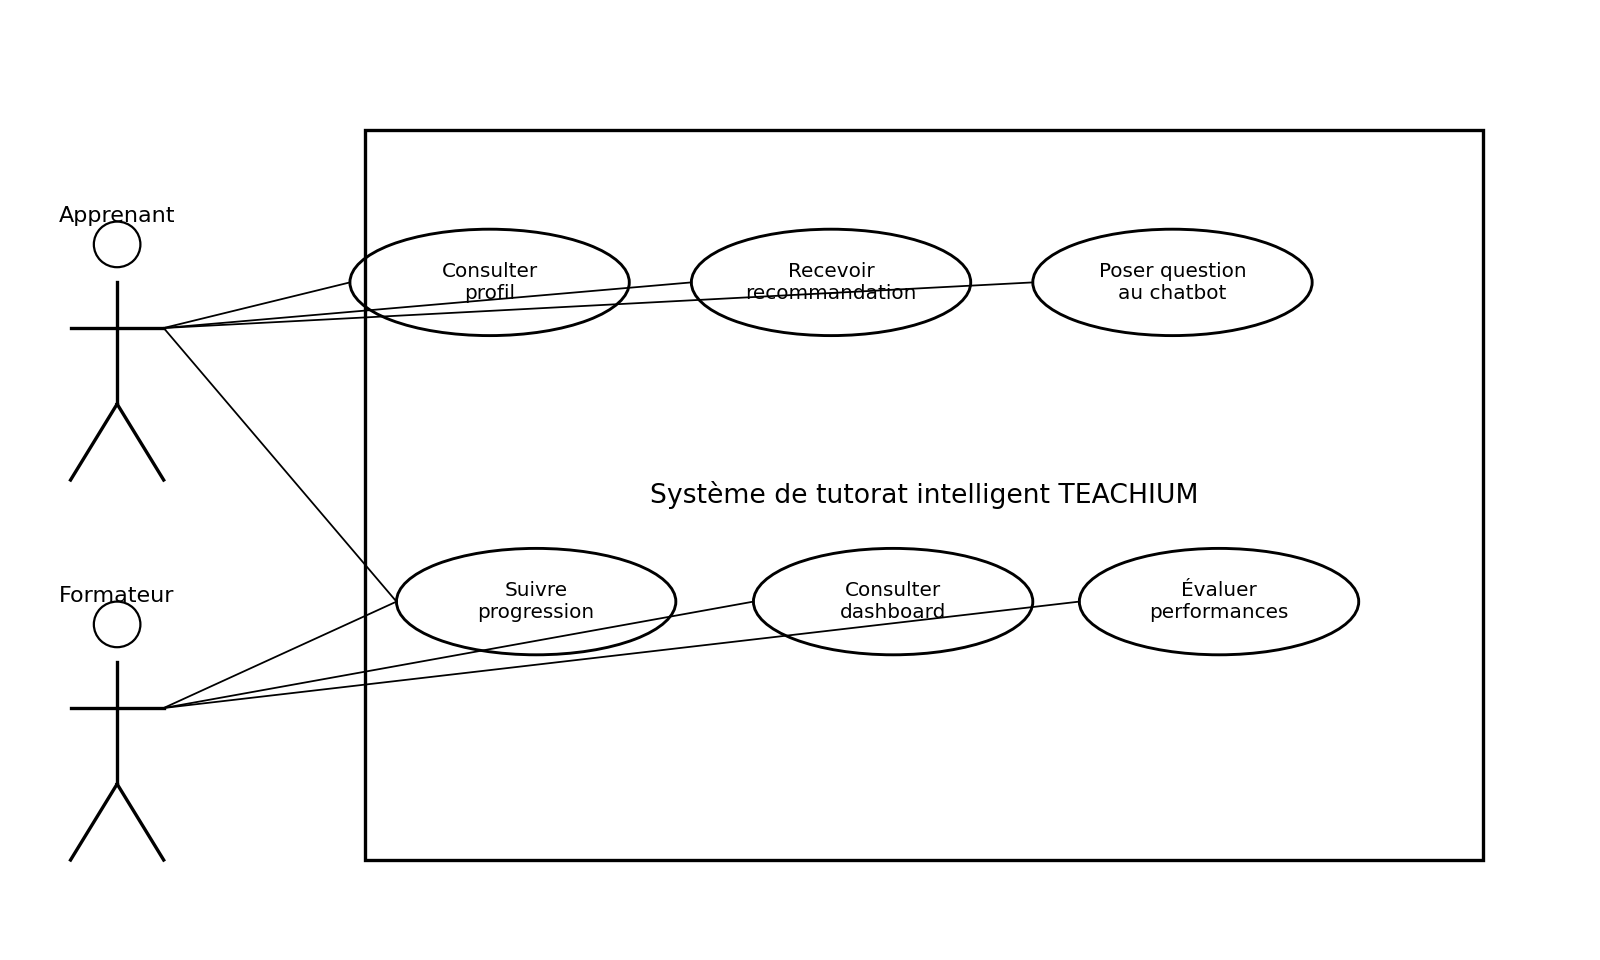
\includegraphics[width=0.9\textwidth]{diagramme_cas_utilisation.png}
\caption{Diagramme de cas d'utilisation du système}
\end{figure}

Le diagramme de cas d'utilisation montre les interactions principales. L'apprenant peut consulter son profil, recevoir une recommandation et poser une question à l'assistant. Le formateur peut suivre la progression à travers le dashboard. L'administrateur peut consulter les performances globales du système.

\section{Diagramme de classes}

\begin{figure}[H]
\centering
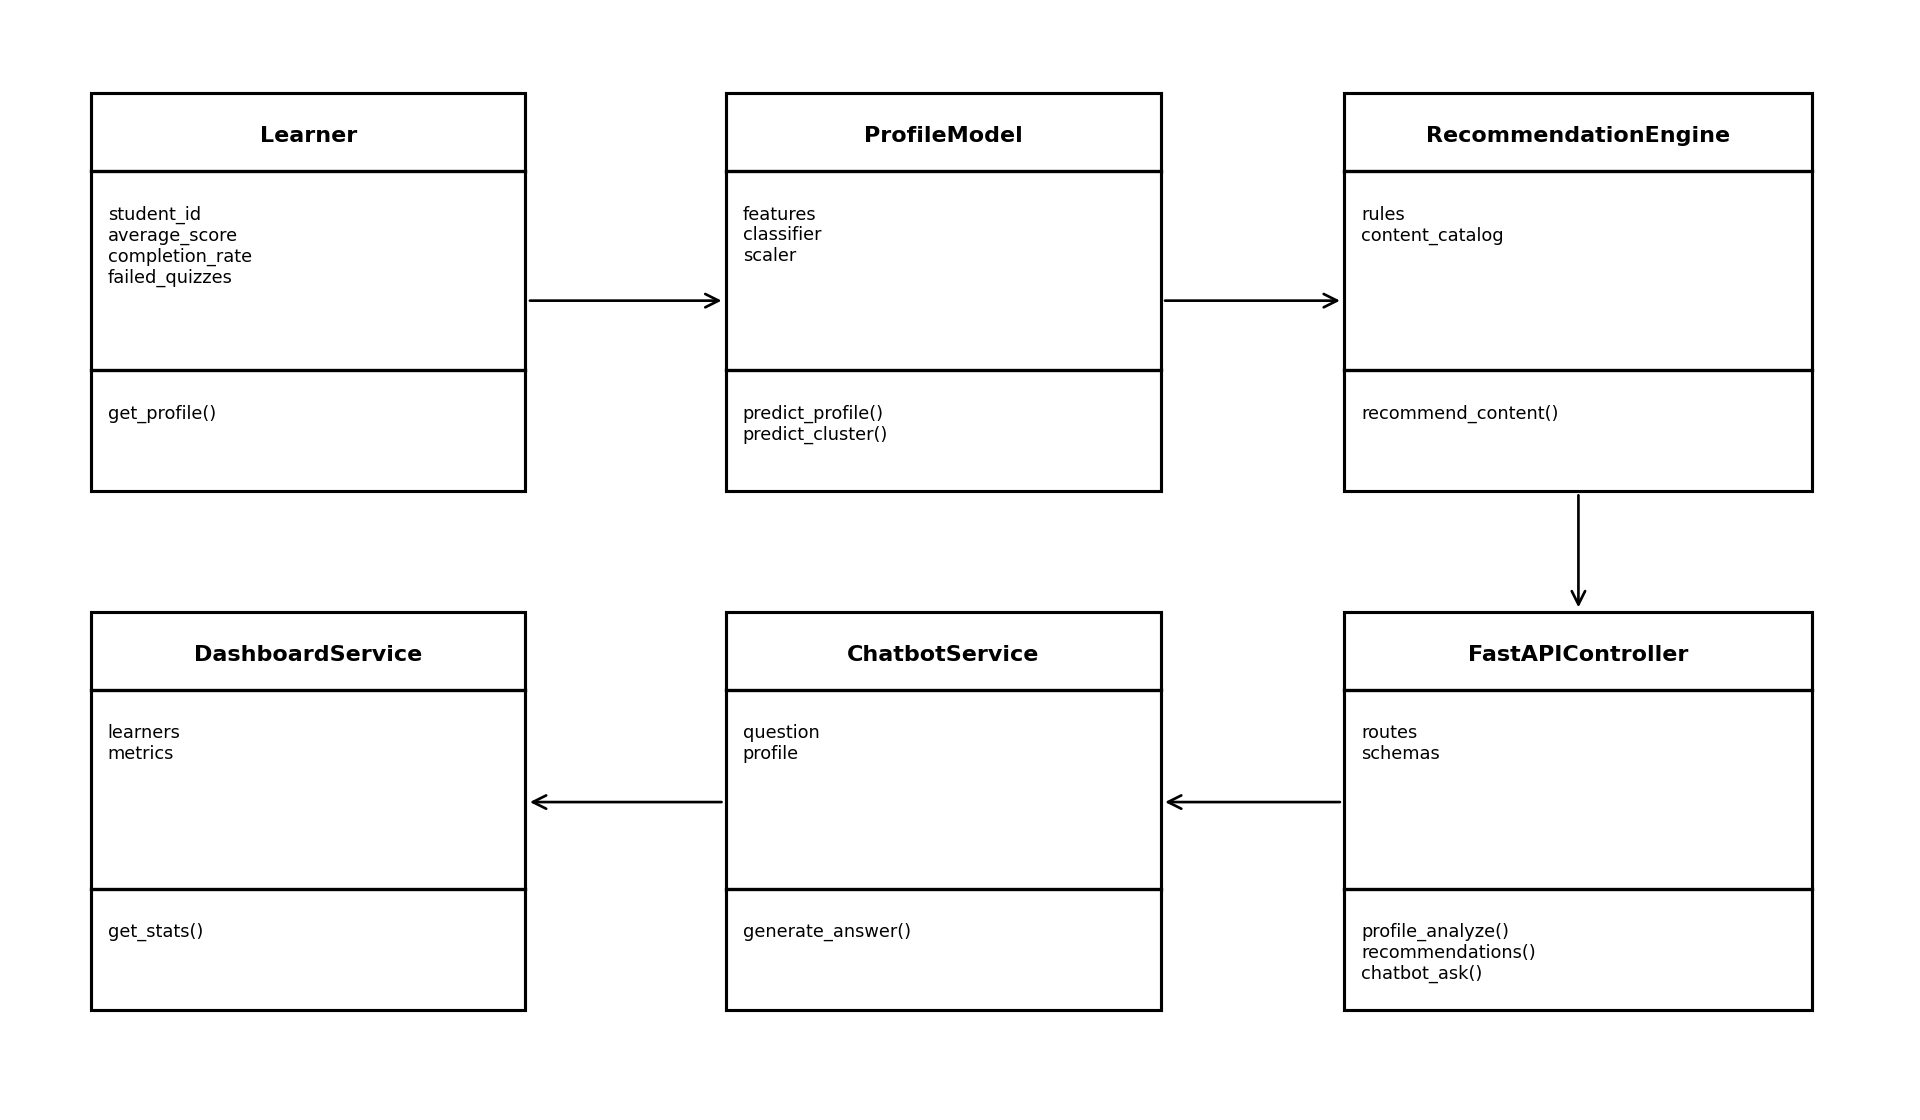
\includegraphics[width=0.95\textwidth]{diagramme_classes.png}
\caption{Diagramme de classes simplifié du prototype}
\end{figure}

Le diagramme de classes présente les principales entités logicielles. La classe \texttt{Learner} représente les données de l'apprenant. Le \texttt{ProfileModel} effectue la prédiction du profil. Le \texttt{RecommendationEngine} génère les recommandations. Le \texttt{ChatbotService} fournit les réponses conversationnelles. Le \texttt{FastAPIController} expose ces fonctionnalités sous forme d'endpoints.

\section{Dictionnaire des données}

\begin{longtable}{|p{4cm}|p{3cm}|p{7cm}|}
\caption{Dictionnaire des données du dataset apprenant}\\
\hline
\textbf{Champ} & \textbf{Type} & \textbf{Description} \\
\hline
\endfirsthead
\hline
\textbf{Champ} & \textbf{Type} & \textbf{Description} \\
\hline
\endhead
student\_id & Chaîne & Identifiant anonyme de l'apprenant. \\
\hline
course\_category & Chaîne & Catégorie principale du contenu suivi. \\
\hline
average\_score & Numérique & Score moyen obtenu dans les quiz. \\
\hline
quiz\_attempts & Entier & Nombre total de quiz passés. \\
\hline
completed\_courses & Entier & Nombre de cours terminés. \\
\hline
total\_courses & Entier & Nombre total de cours affectés à l'apprenant. \\
\hline
time\_spent\_hours & Numérique & Temps passé sur la plateforme en heures. \\
\hline
completion\_rate & Numérique & Pourcentage de complétion du parcours. \\
\hline
login\_frequency & Entier & Nombre moyen de connexions par semaine. \\
\hline
failed\_quizzes & Entier & Nombre de quiz échoués. \\
\hline
satisfaction\_score & Numérique & Note de satisfaction de 1 à 5. \\
\hline
true\_profile & Chaîne & Profil pédagogique simulé utilisé comme cible de classification. \\
\hline
cluster & Entier & Groupe obtenu par K-Means. \\
\hline
profile & Chaîne & Interprétation pédagogique du cluster. \\
\hline
\end{longtable}

\section{Choix des modèles IA et justification}

Le choix de K-Means est justifié par sa simplicité, sa rapidité et sa capacité à regrouper les apprenants sans étiquettes initiales. Il permet de découvrir des profils à partir de plusieurs indicateurs numériques.

Le choix de l'arbre de décision est justifié par son interprétabilité. Dans un contexte pédagogique, il est important de comprendre pourquoi un apprenant est classé comme débutant, moyen, avancé ou en difficulté. Un arbre de décision permet de relier les variables d'entrée aux décisions de manière plus transparente que certains modèles plus complexes.

Le moteur de recommandation est basé sur des règles parce que le stage dure un mois et que les données réelles peuvent être limitées. Cette approche permet de produire rapidement un système cohérent, explicable et évolutif.

\section{Architecture réseau}

L'architecture réseau du prototype est locale. Le backend FastAPI est lancé sur \texttt{localhost:8000}. Le dashboard Streamlit est lancé séparément sur un port local. Dans une intégration future, l'API pourrait être déployée sur un serveur de TEACHIUM et consommée directement par la plateforme LMS.

\section{Modèle BI}

Le modèle BI du prototype repose sur quatre familles d'indicateurs : activité, performance, progression et satisfaction. Ces indicateurs permettent d'alimenter le dashboard et d'aider les formateurs à suivre l'état des apprenants.

\begin{longtable}{|p{4cm}|p{10cm}|}
\caption{Indicateurs BI proposés}\\
\hline
\textbf{Dimension} & \textbf{Indicateurs} \\
\hline
\endfirsthead
\hline
\textbf{Dimension} & \textbf{Indicateurs} \\
\hline
\endhead
Performance & Score moyen, nombre de quiz réussis, nombre de quiz échoués. \\
\hline
Progression & Taux de complétion, nombre de cours terminés. \\
\hline
Activité & Temps passé, fréquence de connexion, nombre de quiz passés. \\
\hline
Satisfaction & Score de satisfaction utilisateur, feedback. \\
\hline
\end{longtable}

\section{Synthèse de la conception}

La conception proposée répond à une logique modulaire. Chaque composant possède un rôle bien défini : le module de données prépare les variables, le module IA détecte le profil, le moteur de recommandation propose les ressources, l'assistant conversationnel explique les résultats et l'API REST assure la communication entre les parties. Cette séparation facilite la maintenance et permet de remplacer un module sans modifier toute l'application.

Cette architecture est également adaptée à une évolution future. Par exemple, le dataset simulé peut être remplacé par une base de données réelle, le moteur de recommandation par règles peut être enrichi par un modèle supervisé, et le chatbot simple peut évoluer vers un assistant LLM connecté aux contenus pédagogiques de TEACHIUM. Le prototype constitue donc une base technique claire pour une intégration progressive dans un environnement e-learning réel.

Du point de vue pédagogique, le système ne se limite pas à prédire un profil. Il explique la décision et propose une action concrète : réviser, pratiquer, reprendre un parcours court ou passer à un niveau avancé. Cette logique rend le système plus utile pour l'apprenant et plus compréhensible pour l'équipe pédagogique.

% ===================== CHAPITRE 5 =====================
\chapter{Implémentation et résultats}

\section{Environnement software et hardware}

Le prototype a été développé dans un environnement Python et peut être ouvert dans Visual Studio Code. Les technologies principales utilisées sont Python, FastAPI, scikit-learn, pandas, matplotlib et Streamlit.

\begin{longtable}{|p{4cm}|p{10cm}|}
\caption{Environnement technique du prototype}\\
\hline
\textbf{Élément} & \textbf{Description} \\
\hline
\endfirsthead
\hline
\textbf{Élément} & \textbf{Description} \\
\hline
\endhead
Éditeur & Visual Studio Code \\
\hline
Langage & Python \\
\hline
Backend & FastAPI \\
\hline
Machine learning & scikit-learn \\
\hline
Données & CSV simulé \\
\hline
Visualisation & matplotlib, Streamlit \\
\hline
Tests & pytest et Swagger \\
\hline
\end{longtable}

\section{Structure du projet}

\begin{lstlisting}[style=pythonstyle,caption={Structure principale du projet}]
teachium_ai_tutor_project/
├── app/
│   ├── main.py
│   ├── schemas/
│   ├── services/
│   ├── models/
│   └── data/
├── dashboard/
│   └── dashboard.py
├── scripts/
│   ├── generate_dataset.py
│   └── train_models.py
├── figures/
├── reports/
│   └── rapport_stage_teachium.tex
├── tests/
├── requirements.txt
└── README.md
\end{lstlisting}

Cette organisation sépare clairement les responsabilités. Le dossier \texttt{app} contient le backend et les services métiers. Le dossier \texttt{scripts} contient les scripts de génération des données et d'entraînement. Le dossier \texttt{dashboard} contient l'interface de suivi. Les figures et le rapport sont séparés afin de faciliter la documentation.

\section{Préparation des données}

En l'absence de données réelles directement exploitables, un dataset simulé a été généré. Ce dataset contient 350 apprenants et plusieurs variables pédagogiques. Les profils simulés sont : avancé, moyen, débutant, en difficulté et peu actif.

\begin{figure}[H]
\centering
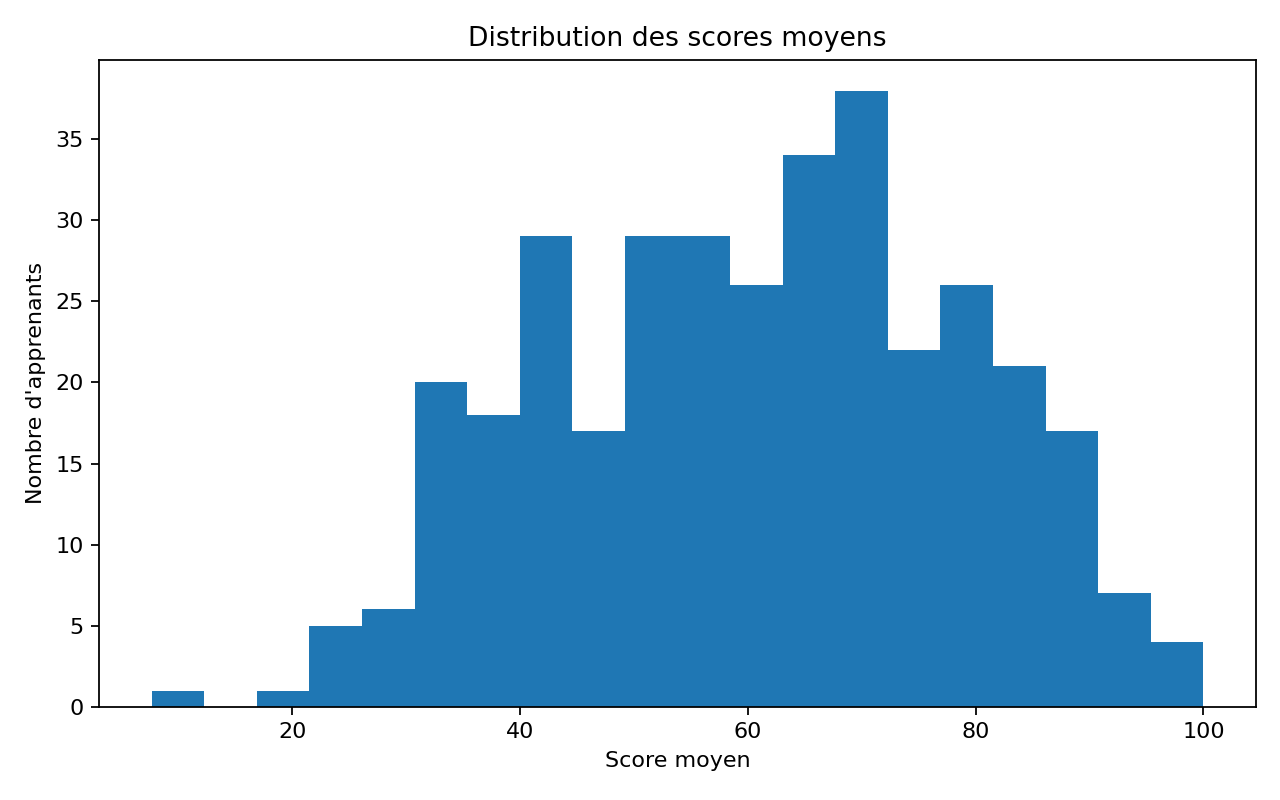
\includegraphics[width=0.8\textwidth]{score_distribution.png}
\caption{Distribution des scores moyens des apprenants}
\end{figure}

La figure montre une distribution variée des scores. Cette diversité est importante pour tester la capacité du système à différencier les profils pédagogiques.

\begin{figure}[H]
\centering
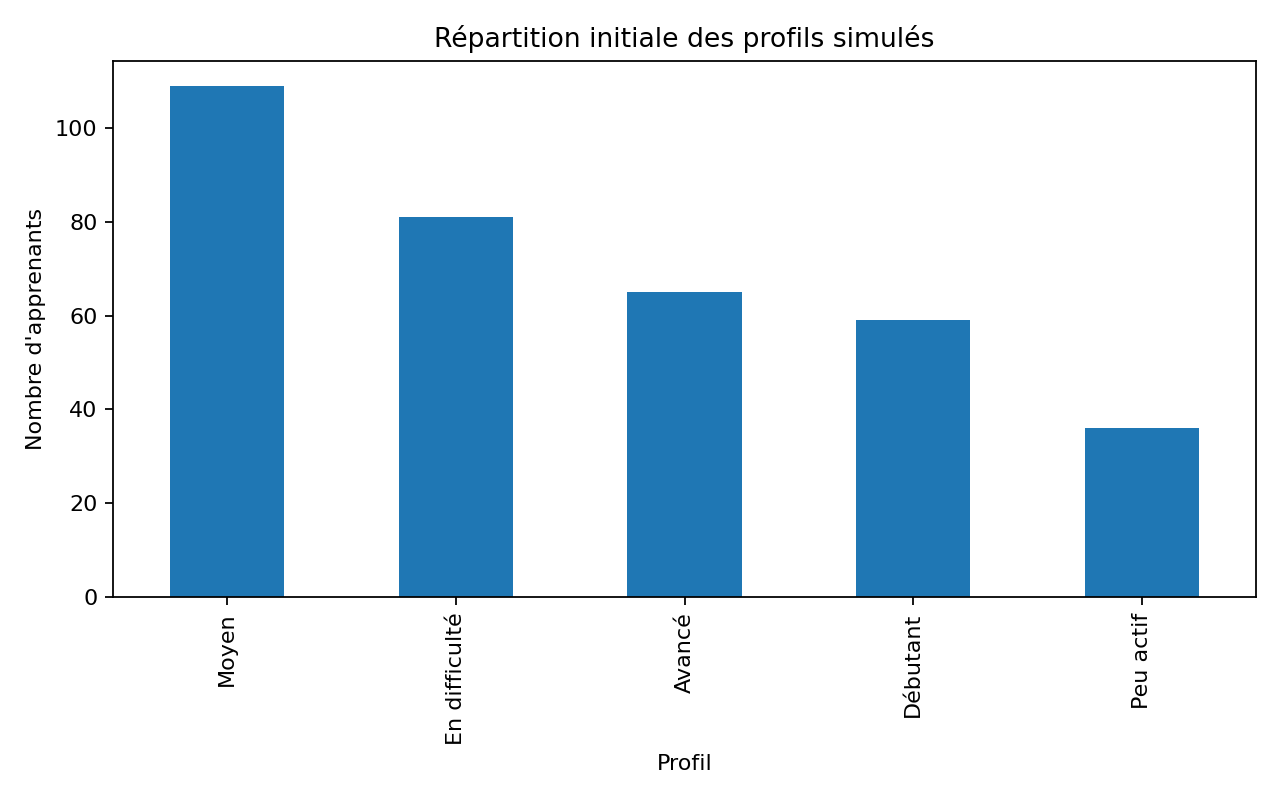
\includegraphics[width=0.8\textwidth]{profiles_distribution.png}
\caption{Répartition des profils apprenants simulés}
\end{figure}

La répartition des profils permet de vérifier que le dataset contient plusieurs catégories d'apprenants. Le système peut ainsi être testé sur des cas différents : apprenants avancés, apprenants moyens, apprenants débutants, apprenants en difficulté et apprenants peu actifs.

\begin{figure}[H]
\centering
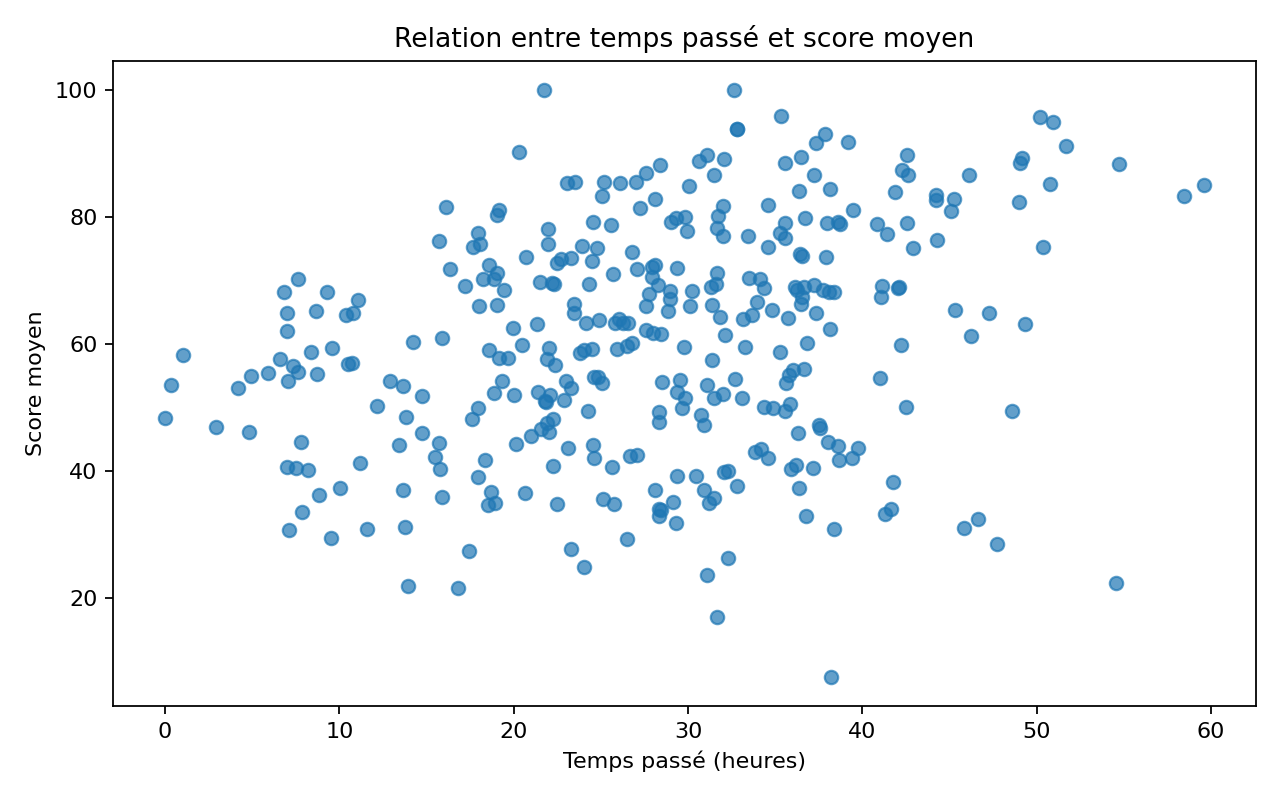
\includegraphics[width=0.8\textwidth]{score_vs_time.png}
\caption{Relation entre le temps passé et le score moyen}
\end{figure}

Cette visualisation permet d'observer la relation entre l'engagement et la performance. Un temps élevé ne garantit pas toujours un score élevé, ce qui justifie l'utilisation de plusieurs indicateurs pour définir un profil.

\section{Clustering des apprenants}

Le clustering a été réalisé avec K-Means après normalisation des variables numériques. La méthode Elbow a été utilisée pour observer l'évolution de l'inertie selon le nombre de clusters.

\begin{figure}[H]
\centering
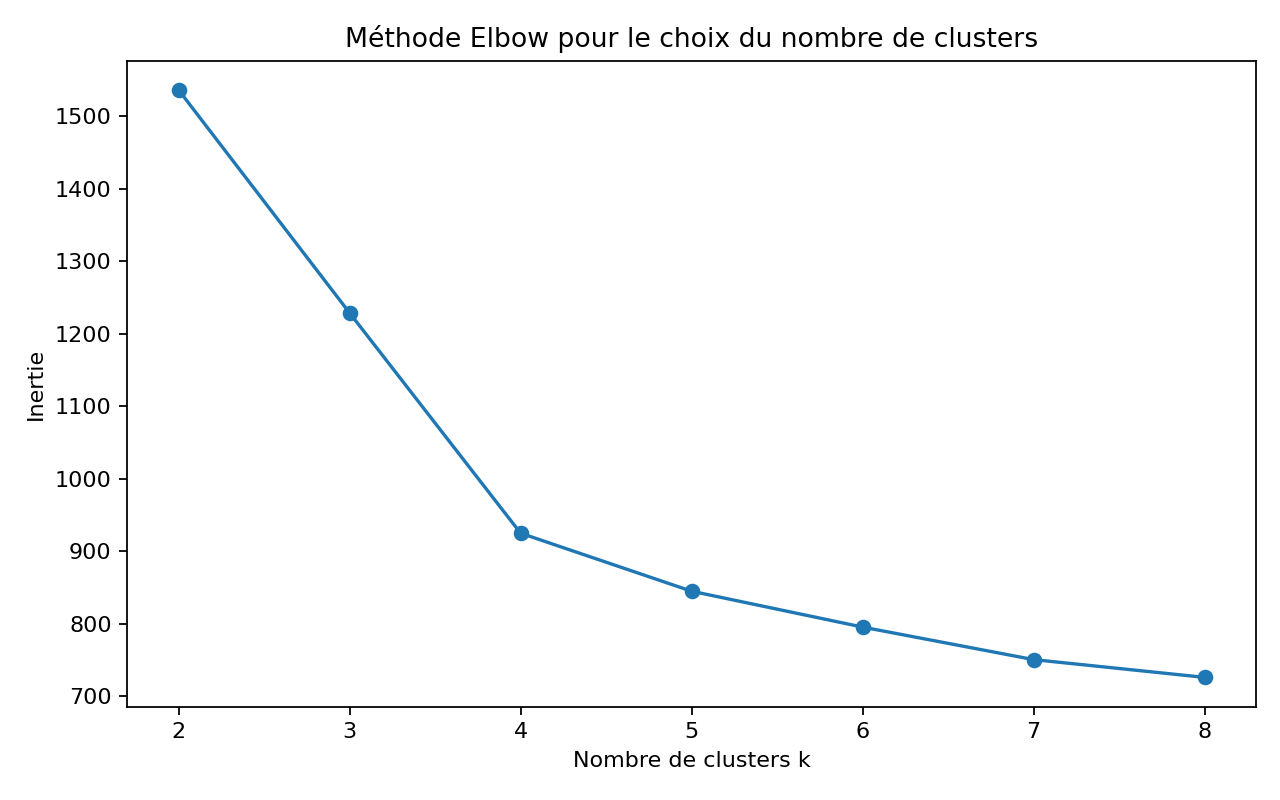
\includegraphics[width=0.8\textwidth]{elbow_method.png}
\caption{Méthode Elbow pour le choix du nombre de clusters}
\end{figure}

La figure montre l'évolution de l'inertie lorsque le nombre de clusters augmente. Pour ce prototype, cinq clusters ont été retenus afin de correspondre aux cinq profils pédagogiques principaux.

\section{Classification par arbre de décision}

Un modèle \texttt{DecisionTreeClassifier} a été entraîné pour prédire le profil d'un apprenant à partir des variables pédagogiques. Les variables utilisées sont le score moyen, le temps passé, le taux de complétion, le nombre de quiz passés, le nombre de quiz échoués, la fréquence de connexion et la satisfaction.

\begin{figure}[H]
\centering
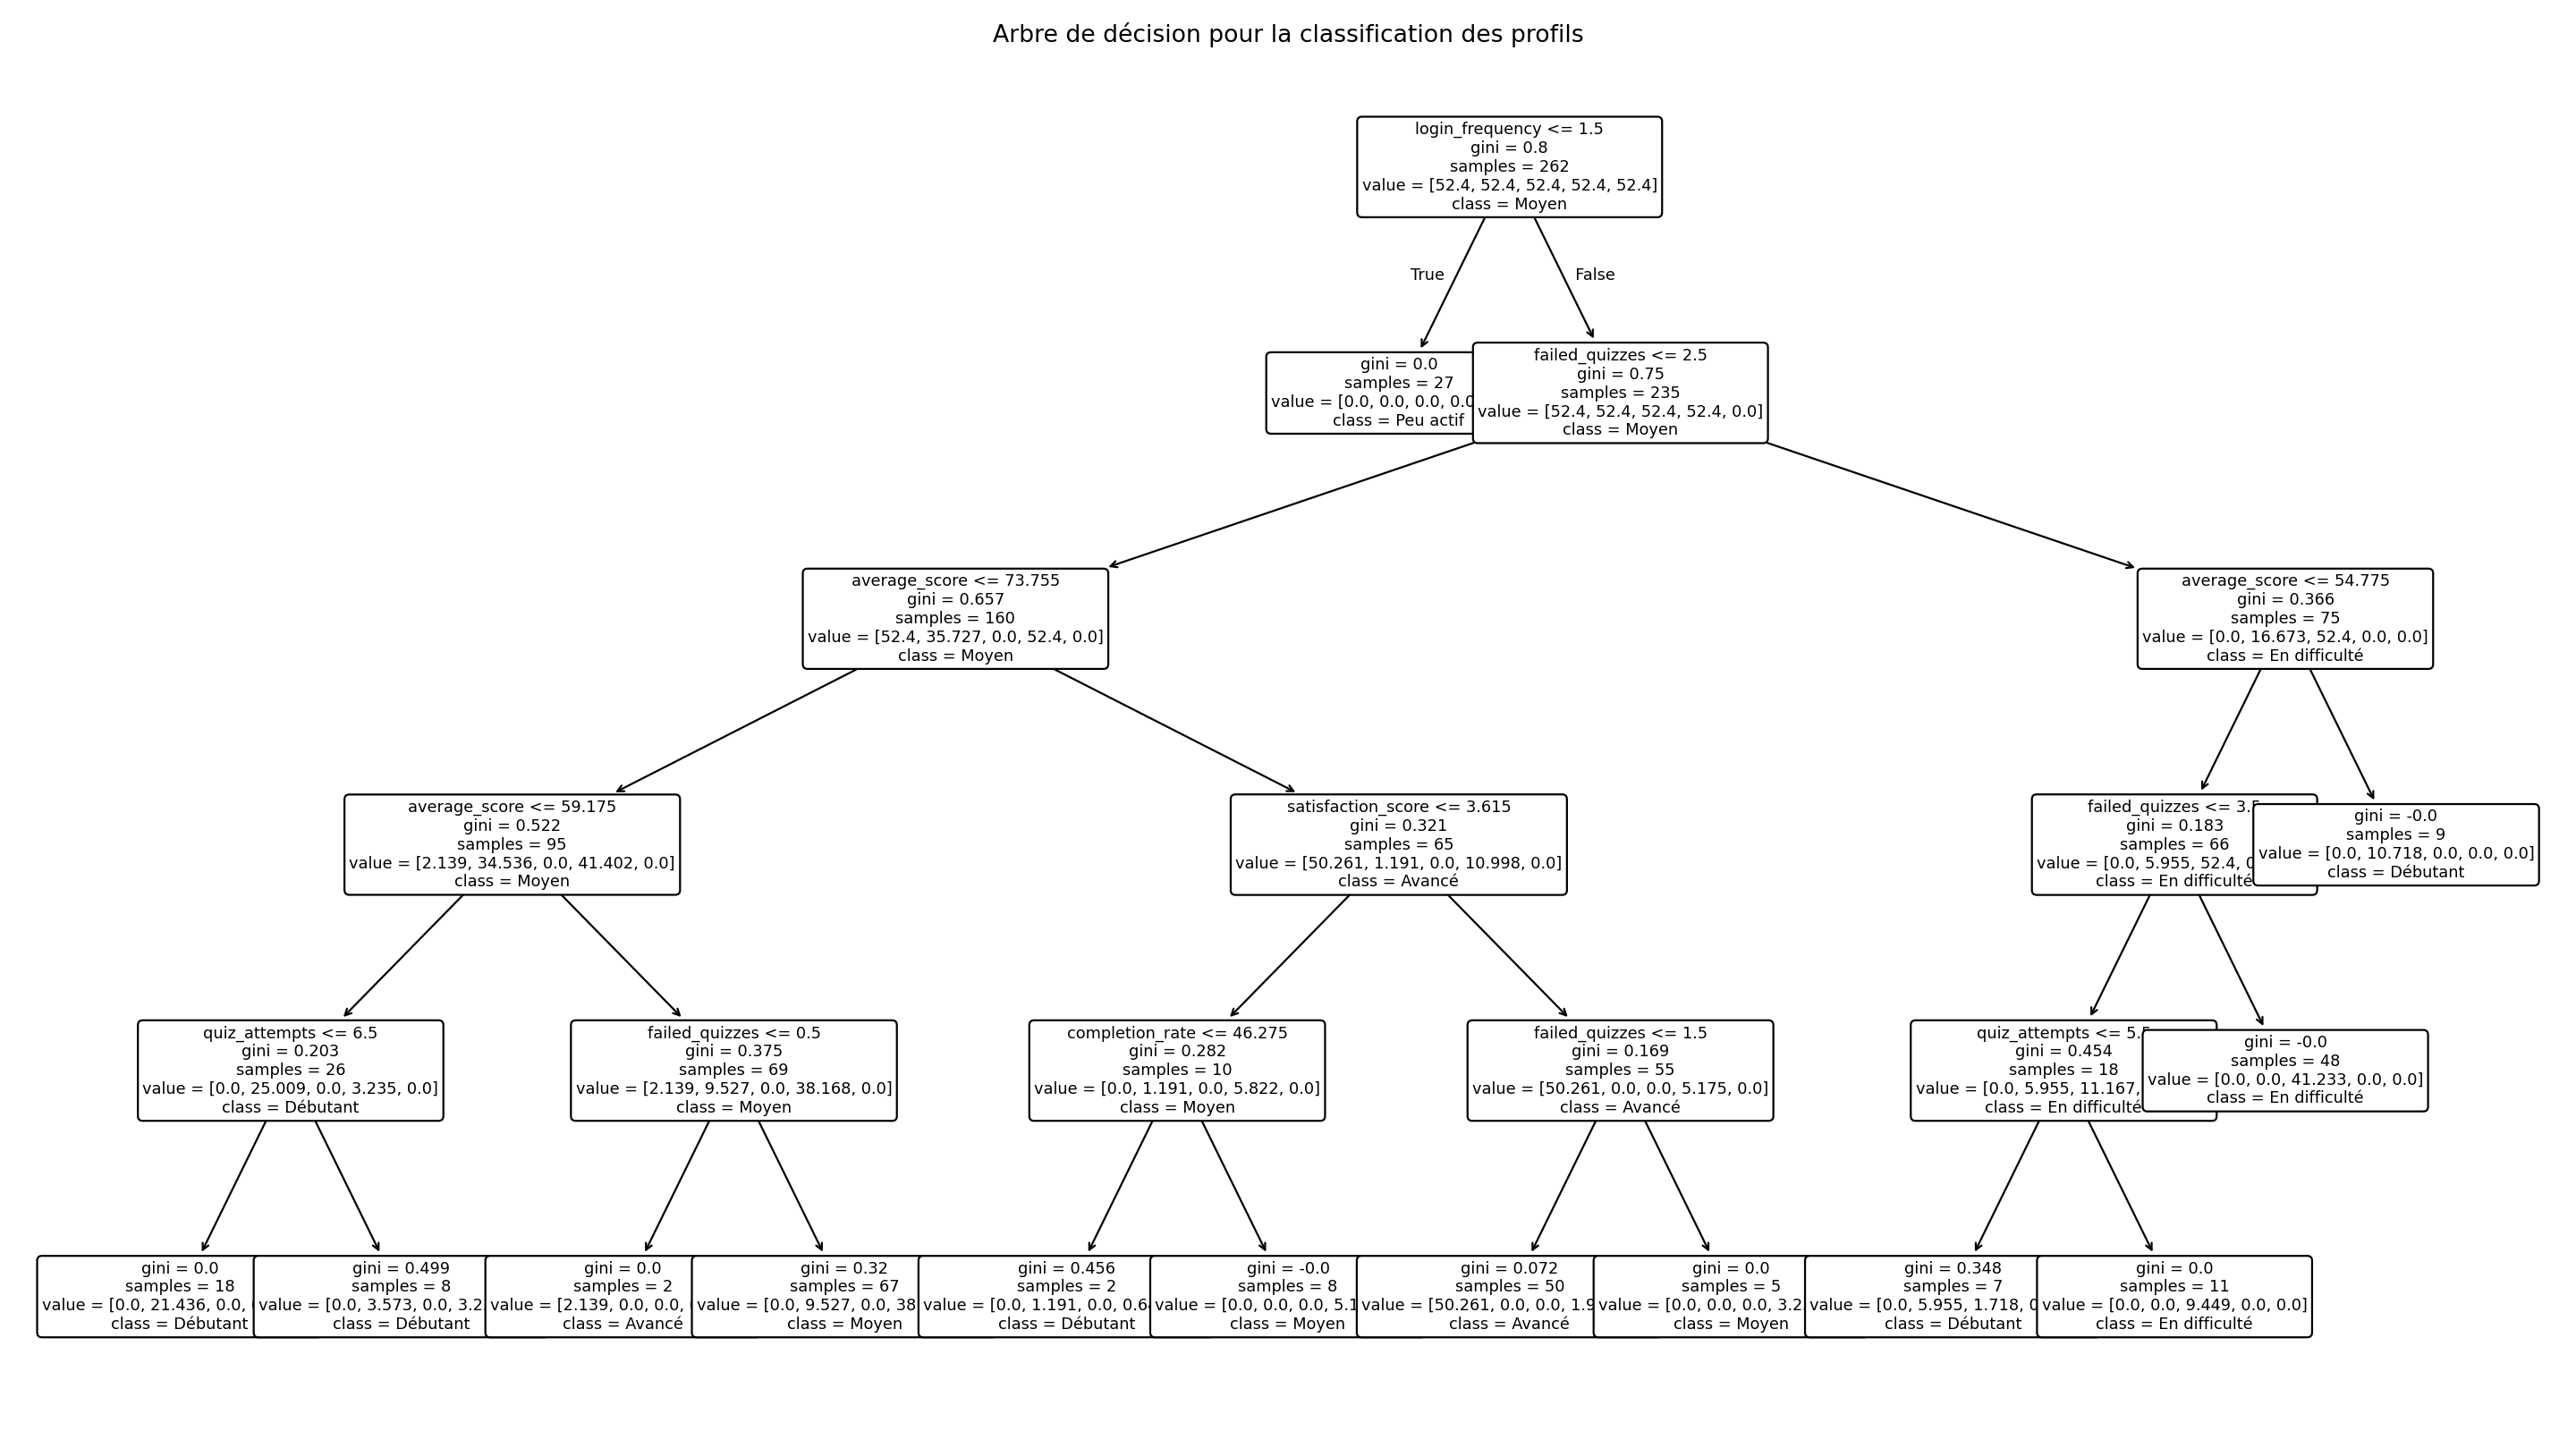
\includegraphics[width=0.95\textwidth]{decision_tree.png}
\caption{Arbre de décision entraîné pour la classification des profils}
\end{figure}

L'arbre de décision permet d'interpréter les décisions du modèle. Il montre que les variables comme le score moyen, la complétion et les quiz échoués jouent un rôle important dans la séparation des profils.

\section{Résultats d'évaluation}

Le modèle de classification a été évalué sur un jeu de test représentant 25\% du dataset. Les résultats obtenus sont présentés dans le tableau suivant.

\begin{table}[H]
\centering
\caption{Métriques globales du modèle de classification}
\begin{tabular}{|p{5cm}|p{4cm}|}
\hline
\textbf{Métrique} & \textbf{Valeur} \\
\hline
Accuracy & 0.8409 \\
\hline
Precision pondérée & 0.8610 \\
\hline
Recall pondéré & 0.8409 \\
\hline
F1-score pondéré & 0.8459 \\
\hline
\end{tabular}
\end{table}

Ces résultats montrent que le modèle parvient à reconnaître correctement la majorité des profils simulés. Les performances sont satisfaisantes pour un prototype, mais elles doivent être interprétées avec prudence car les données sont simulées.

\begin{figure}[H]
\centering
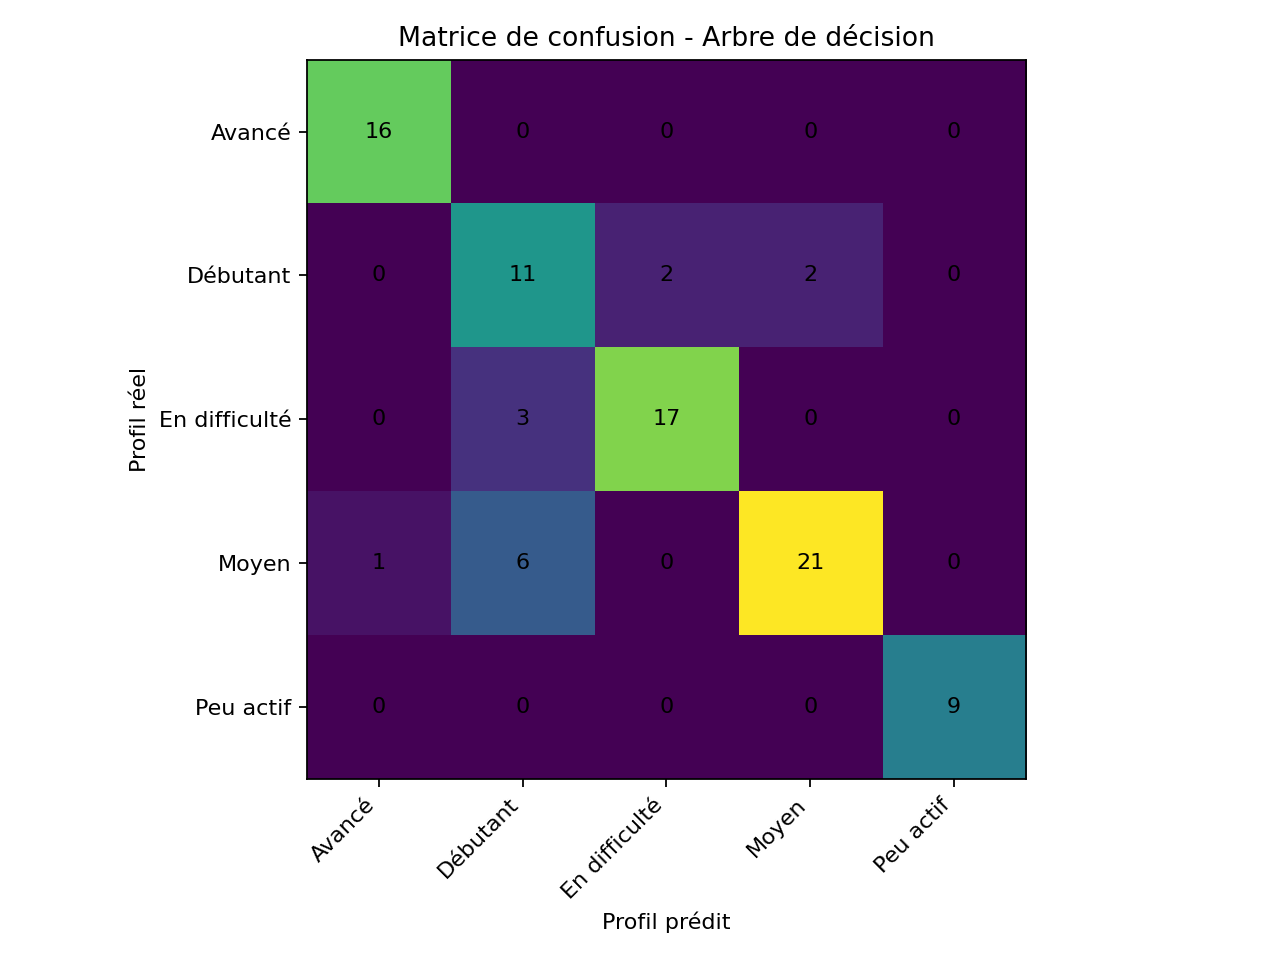
\includegraphics[width=0.8\textwidth]{confusion_matrix.png}
\caption{Matrice de confusion du modèle de classification}
\end{figure}

La matrice de confusion permet d'identifier les confusions entre profils. Les profils les plus distincts, comme \textit{Avancé} et \textit{Peu actif}, sont mieux reconnus. Les profils intermédiaires, comme \textit{Débutant} et \textit{Moyen}, peuvent être plus proches et donc plus difficiles à séparer.

\section{Moteur de recommandation}

Le moteur de recommandation repose sur des règles pédagogiques simples. Ces règles associent chaque profil à un type de contenu adapté.

\begin{longtable}{|p{4cm}|p{10cm}|}
\caption{Exemples de recommandations pédagogiques}\\
\hline
\textbf{Profil} & \textbf{Recommandation} \\
\hline
\endfirsthead
\hline
\textbf{Profil} & \textbf{Recommandation} \\
\hline
\endhead
En difficulté & Cours de révision, vidéo explicative, quiz de renforcement. \\
\hline
Débutant & Module d'introduction, exercices guidés, quiz facile. \\
\hline
Moyen & Exercices standards, quiz de progression, résumé de cours. \\
\hline
Avancé & Contenu avancé, mini-projet pratique, quiz supérieur. \\
\hline
Peu actif & Parcours court, rappel motivationnel, objectif hebdomadaire simple. \\
\hline
\end{longtable}

Cette approche est simple, mais elle présente un avantage important : elle est explicable. L'équipe pédagogique peut comprendre pourquoi une ressource a été proposée à un apprenant.

\section{API REST}

Les fonctionnalités du système sont exposées à travers une API REST développée avec FastAPI. Les endpoints principaux sont présentés ci-dessous.

\begin{longtable}{|p{5cm}|p{9cm}|}
\caption{Endpoints principaux de l'API}\\
\hline
\textbf{Endpoint} & \textbf{Description} \\
\hline
\endfirsthead
\hline
\textbf{Endpoint} & \textbf{Description} \\
\hline
\endhead
\texttt{GET /} & Vérifie que l'API fonctionne. \\
\hline
\texttt{POST /api/profile/analyze} & Analyse les données d'un apprenant et retourne son profil. \\
\hline
\texttt{POST /api/recommendations} & Retourne des recommandations selon le profil. \\
\hline
\texttt{POST /api/chatbot/ask} & Répond à une question posée à l'assistant. \\
\hline
\texttt{GET /api/dashboard/stats} & Retourne les statistiques du dashboard. \\
\hline
\texttt{GET /api/model/evaluate} & Retourne les métriques d'évaluation du modèle. \\
\hline
\end{longtable}

\section{Assistant conversationnel}

L'assistant conversationnel est une première version fondée sur des mots-clés. Il peut répondre à des questions concernant le profil, les recommandations, les conseils de progression ou les cours à revoir. Cette approche constitue une base simple qui pourra être remplacée par un assistant LLM dans une version future.

\begin{lstlisting}[style=pythonstyle,caption={Exemple simplifié de réponse conversationnelle}]
def chatbot_response(question, profile, recommended_content=None):
    q = question.lower()
    if "profil" in q:
        return f"Votre profil actuel est : {profile}."
    if "recommand" in q:
        return "Cette ressource est recommandée selon votre profil."
    return "Je peux vous aider à comprendre votre parcours."
\end{lstlisting}

\section{Dashboard}

Un dashboard Streamlit a été développé pour visualiser les données et tester le prototype. Il affiche le nombre d'apprenants, le score moyen, le taux de complétion moyen, la satisfaction moyenne, la répartition des profils et des graphiques exploratoires.

Le dashboard contient également un formulaire permettant de saisir les données d'un apprenant et d'obtenir automatiquement son profil et ses recommandations. Cela facilite la démonstration du système auprès de l'encadrant.

\section{Tests réalisés}

Les tests ont porté sur les endpoints de l'API, le fonctionnement du moteur de recommandation et l'analyse de profil. Les tests unitaires simples ont été réalisés avec \texttt{pytest}.

\begin{table}[H]
\centering
\caption{Résumé des tests fonctionnels}
\begin{tabular}{|p{4cm}|p{5cm}|p{3cm}|}
\hline
\textbf{Test} & \textbf{Résultat attendu} & \textbf{Statut} \\
\hline
Route racine & Message de fonctionnement de l'API & Validé \\
\hline
Analyse profil & Retour d'un profil pédagogique & Validé \\
\hline
Recommandation & Liste de contenus recommandés & Validé \\
\hline
Chatbot & Réponse textuelle adaptée & Validé \\
\hline
Dashboard & Affichage des indicateurs & Validé \\
\hline
\end{tabular}
\end{table}

\section{Discussion des résultats avec SWOT}

\begin{longtable}{|p{3cm}|p{11cm}|}
\caption{Analyse SWOT du prototype}\\
\hline
\textbf{Élément} & \textbf{Analyse} \\
\hline
\endfirsthead
\hline
\textbf{Élément} & \textbf{Analyse} \\
\hline
\endhead
Forces & Architecture claire, prototype fonctionnel, API testable, résultats interprétables, dashboard simple. \\
\hline
Faiblesses & Données simulées, chatbot limité, recommandation basée sur des règles, absence d'intégration réelle avec un LMS. \\
\hline
Opportunités & Intégration avec les données réelles de TEACHIUM, amélioration par LLM, personnalisation plus avancée, suivi pédagogique en temps réel. \\
\hline
Menaces & Qualité insuffisante des données, contraintes de confidentialité, coût d'un LLM, difficulté d'intégration avec l'existant. \\
\hline
\end{longtable}

% ===================== CONCLUSION =====================
\chapter*{Conclusion générale et perspectives}
\addcontentsline{toc}{chapter}{Conclusion générale et perspectives}

Ce stage a permis de concevoir et développer un prototype de système de tutorat intelligent basé sur l'intelligence artificielle pour la personnalisation des parcours d'apprentissage. Le système réalisé répond aux objectifs principaux : analyser les données d'un apprenant, détecter son profil pédagogique, générer des recommandations adaptées, fournir une assistance conversationnelle simple et afficher les indicateurs dans un dashboard.

Les résultats obtenus montrent qu'une première version fonctionnelle est réalisable dans le cadre d'un stage d'un mois. Le modèle de classification atteint une accuracy de 0.8409 sur les données simulées, ce qui constitue un résultat satisfaisant pour un prototype. Le moteur de recommandation permet de relier chaque profil à des ressources pédagogiques adaptées, tandis que l'API REST rend le système testable et intégrable.

L'impact potentiel pour TEACHIUM est important. Une telle solution peut aider l'entreprise à enrichir ses services e-learning par une personnalisation plus fine, un meilleur suivi des apprenants et une aide intelligente à la décision pédagogique. Pour la formation personnelle du stagiaire, ce projet a permis de mobiliser des compétences en développement backend, machine learning, visualisation de données, conception logicielle et documentation technique.

Cependant, le prototype présente certaines limites. Les données utilisées sont simulées et ne remplacent pas des données réelles. Le chatbot reste simple et ne comprend pas réellement le contenu des cours. Le moteur de recommandation est basé sur des règles et non sur un historique réel d'interactions. Ces limites constituent des axes d'amélioration pour une version future.

Les perspectives possibles sont l'intégration de données réelles anonymisées, l'utilisation d'un modèle LLM connecté aux supports pédagogiques de TEACHIUM, l'amélioration du moteur de recommandation par apprentissage, l'ajout d'un système de feedback utilisateur et le déploiement de l'API sur un serveur de production.

% ===================== REFERENCES =====================
\chapter*{Références bibliographiques}
\addcontentsline{toc}{chapter}{Références bibliographiques}

\begin{thebibliography}{9}

\bibitem{sklearn-kmeans}
Scikit-learn, \textit{KMeans - scikit-learn documentation}. Disponible sur : \url{https://scikit-learn.org/stable/modules/generated/sklearn.cluster.KMeans.html}. Consulté en 2026.

\bibitem{sklearn-tree}
Scikit-learn, \textit{Decision Trees - scikit-learn documentation}. Disponible sur : \url{https://scikit-learn.org/stable/modules/tree.html}. Consulté en 2026.

\bibitem{fastapi-docs}
FastAPI, \textit{FastAPI documentation - Features}. Disponible sur : \url{https://fastapi.tiangolo.com/features/}. Consulté en 2026.

\bibitem{streamlit-docs}
Streamlit, \textit{Get started with Streamlit - Streamlit Docs}. Disponible sur : \url{https://docs.streamlit.io/get-started}. Consulté en 2026.

\bibitem{rag-lewis}
P. Lewis, E. Perez, A. Piktus et al., \textit{Retrieval-Augmented Generation for Knowledge-Intensive NLP Tasks}, arXiv:2005.11401, 2020.

\bibitem{teachium-official}
TEACHIUM, \textit{Site web officiel}. Disponible sur : \url{https://www.teachium.com}. Consulté en 2026.

\end{thebibliography}

% ===================== ANNEXES =====================
\appendix
\chapter{Commandes d'exécution du projet}

\begin{lstlisting}[style=pythonstyle,caption={Installation et lancement du projet}]
python -m venv .venv
.\.venv\Scripts\Activate.ps1
pip install -r requirements.txt
python scripts/generate_dataset.py
python scripts/train_models.py
uvicorn app.main:app --reload
streamlit run dashboard/dashboard.py
\end{lstlisting}

\chapter{Exemple de requête API}

\begin{lstlisting}[style=pythonstyle,caption={Payload JSON pour l'analyse d'un apprenant}]
{
  "average_score": 45,
  "time_spent_hours": 12,
  "completion_rate": 40,
  "quiz_attempts": 5,
  "failed_quizzes": 3,
  "login_frequency": 2,
  "satisfaction_score": 2.5
}
\end{lstlisting}

\chapter{Limites techniques}

Le prototype ne remplace pas une plateforme LMS complète. Il constitue une preuve de concept. Pour une mise en production, il serait nécessaire d'ajouter une authentification, une base de données robuste, une gestion des droits, un système de logs, une stratégie de confidentialité des données et une intégration réelle avec l'environnement technique de TEACHIUM.

\end{document}
